% Figure 1 with its innermost box opened out: the Rollout Oracle, drawn in
% the deck's green, unfolds beneath into the factors of Theorem 3's
% composition, U_index and U_trans for rounds 1 to H, then U_eval.  The
% Figure 1 half is fig1.tex's tikzpicture verbatim, save the colour of the
% one box; the Makefile renders the whole to an SVG of paths.
\documentclass[dvisvgm]{standalone}
\usepackage{amsmath,amssymb}
\usepackage{tikz}
\usetikzlibrary{decorations.pathreplacing}
\definecolor{deckgreen}{HTML}{4D8C55}
\tikzset{phase/.style={draw=deckgreen, fill=deckgreen!12, rounded corners=2pt,
  line width=0.4mm, minimum width=1.25cm, minimum height=0.6cm, font=\footnotesize}}
\begin{document}
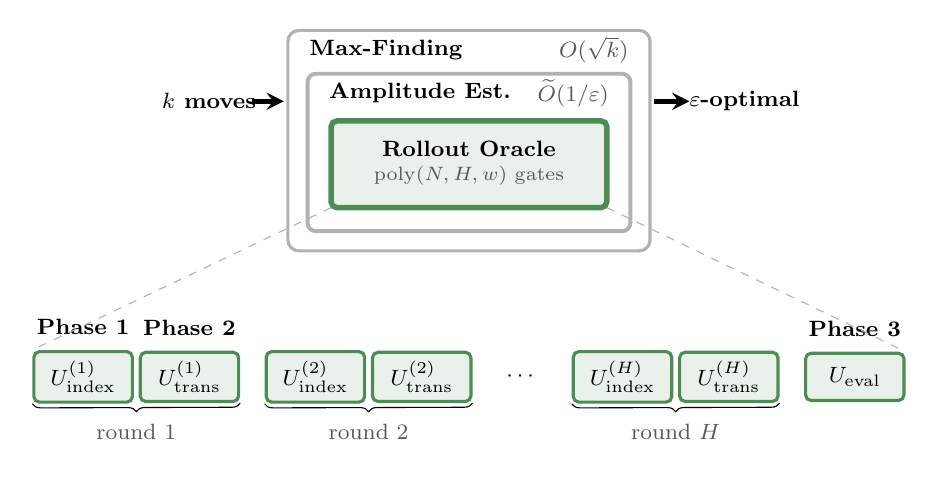
\begin{tikzpicture}[
  lbl/.style={font=\footnotesize},
  cost/.style={font=\footnotesize, text=gray!70!black},
  arr/.style={->, >=stealth, line width=0.6mm},
]
  % ── Input: k moves (text only) ──
  \node[lbl, font=\footnotesize\bfseries] at (0, -0.9) {$k$ moves};

  % arrow to Level 1
  \draw[arr] (0.55, -0.9) -- (0.95, -0.9);

  % ── Level 1: Max-Finding ──
  \draw[rounded corners=4pt, line width=0.4mm, gray!60]
    (1.0, 0.0) rectangle (5.6, -2.8);
  \node[lbl, font=\footnotesize\bfseries, anchor=west]
    at (1.15, -0.25) {Max-Finding};
  \node[cost, anchor=east] at (5.45, -0.25) {$O(\sqrt{k})$};

  % ── Level 2: Coherent Amplitude Estimation ──
  \draw[rounded corners=3pt, line width=0.5mm, gray!60]
    (1.25, -0.55) rectangle (5.35, -2.55);
  \node[lbl, font=\footnotesize\bfseries, anchor=west]
    at (1.4, -0.8) {Amplitude Est.};
  \node[cost, anchor=east] at (5.2, -0.8) {$\widetilde{O}(1/\varepsilon)$};

  % ── Level 3: Rollout Oracle (single block) ──
  \draw[fill=deckgreen!12, draw=deckgreen, rounded corners=2pt, line width=0.7mm]
    (1.55, -1.15) rectangle (5.05, -2.25);
  \node[lbl, font=\footnotesize\bfseries] at (3.3, -1.5)
    {Rollout Oracle};
  \node[cost, font=\scriptsize] at (3.3, -1.85)
    {$\mathrm{poly}(N, H, w)$ gates};

  % ── Output: ε-optimal (text only) ──
  \node[lbl, font=\footnotesize\bfseries] at (6.8, -0.9) {$\varepsilon$-optimal};

  % arrow from Level 1 to output
  \draw[arr] (5.65, -0.9) -- (6.1, -0.9);


  % ── The box, opened out: one call is H rounds, then the evaluation ──
  \node[phase] (i1) at (-1.6, -4.4)  {$U^{(1)}_{\mathrm{index}}$};
  \node[phase] (t1) at (-0.25, -4.4) {$U^{(1)}_{\mathrm{trans}}$};
  \node[phase] (i2) at (1.35, -4.4)  {$U^{(2)}_{\mathrm{index}}$};
  \node[phase] (t2) at (2.7, -4.4)   {$U^{(2)}_{\mathrm{trans}}$};
  \node[lbl]        at (3.975, -4.4) {$\cdots$};
  \node[phase] (iH) at (5.25, -4.4)  {$U^{(H)}_{\mathrm{index}}$};
  \node[phase] (tH) at (6.6, -4.4)   {$U^{(H)}_{\mathrm{trans}}$};
  \node[phase] (ev) at (8.2, -4.4)   {$U_{\mathrm{eval}}$};

  \node[lbl, font=\footnotesize\bfseries] at (i1.north) [above=2pt] {Phase 1};
  \node[lbl, font=\footnotesize\bfseries] at (t1.north) [above=2pt] {Phase 2};
  \node[lbl, font=\footnotesize\bfseries] at (ev.north) [above=2pt] {Phase 3};

  \draw[decorate, decoration={brace, mirror, amplitude=3pt}]
    (i1.south west) -- (t1.south east) node[midway, below=4pt, cost] {round 1};
  \draw[decorate, decoration={brace, mirror, amplitude=3pt}]
    (i2.south west) -- (t2.south east) node[midway, below=4pt, cost] {round 2};
  \draw[decorate, decoration={brace, mirror, amplitude=3pt}]
    (iH.south west) -- (tH.south east) node[midway, below=4pt, cost] {round $H$};

  % callout from the box's bottom corners to the strip's top corners
  \draw[dashed, gray!60] (1.55, -2.25) -- (i1.north west);
  \draw[dashed, gray!60] (5.05, -2.25) -- (ev.north east);
\end{tikzpicture}
\end{document}
